\cotefile{1}
\scanpage{92}

En effet, $\overset{\inserted{30}}{27}$ est un cas particulier du th. 2, et ($\overset{\inserted{31}}{28}$) en dérive par passage à la limite pour $n\to+\infty$. \inserted{\textcolor{red!75!black}{$*$}} \deleted{En particulier, prenant $f(\unsure{r|s})=\unsure{r|s}^{\unsure{p|r}}$, $\unsure{p|r}>0$, on obtient} \inserted{Pour un autre cas particulier du corollaire 1,} soient $p,q,\deleted{\unsure{r}}s$ tels que

\reversemarginpar
\margin{\inserted{Prenons en particulier $f(s)\equiv1$, on obtient alors
\(\begingroup
\setbox0=\hbox{$\displaystyle\sum\rho_i(uv)\leq\sum\rho_i(u)\rho_i(v)$}
\textcircled{32}\quad\smash{\rlap{\begin{tikzpicture}[x=\wd0,y=1ex,baseline=0pt]
\draw[red!75!black,line width=.8pt] (-.02,2.2)--(1.04,1.9);
\draw[red!75!black,line width=.8pt] (-.025,1.8)--(-.04,-1.7)--(1.05,-2.0)--(1.04,1.9);
\end{tikzpicture}}}\box0\endgroup\)\unsure{:|.}
Tenant compte du \deleted{(21)} \inserted{N\textsuperscript{o} 1, th. 3}, pour $p=1$, \deleted{et \unsure{soit}} \inserted{on en conclut} que si le deuxième mb est fini, alors $uv$ est un op. de Fredholm. \deleted{Par \unsure{conséquent}} Or si \deleted{\unsure{$\sum\lambda_i$}} \inserted{$E=G$}, on a
\deleted{d'où $|\mathrm{Tr}(uv)|\leq\sum|\lambda_i(uv)|\leq\sum\rho_i(uv)$}
$|\mathrm{Tr}\,uv|\leq\deleted{\unsure{\sum\rho_i(v)|\sum}}\inserted{\sum\rho_i(uv)}$
\deleted{(\unsure{inégalité} \unsure{fond.} (21), pour $p=1$) d'où $|\mathrm{Tr}\,uv|\leq\sum\rho_i(u)\rho_i(v)$. Par \unsure{suite} \unsure{on a}}
\deleted{(N\textsuperscript{o} 2, \unsure{th.})} \inserted{(N\textsuperscript{o} 1, th. \unsure{3|2})}.
\uline{Corollaire 2}. Soient $E,F$ deux espaces de Hilbert, $u$ une application lin. \unsure{cpt|cpte} de $E$ dans $F$, $v$ une application lin. \unsure{cpt|cpte} de $F$ dans $G$, supposons $\sum\rho_i(u)\rho_i(v)<+\infty$, alors $vu$ est un op. de Fredholm, et on a
\(\begingroup
\setbox0=\hbox{$\displaystyle\begin{array}{ll}(33)&|\mathrm{Tr}\,uv|\leq\sum\rho_i(u)\rho_i(v)\\&\deleted{\illegible{3}}\end{array}$}
\smash{\rlap{\begin{tikzpicture}[x=\wd0,y=1ex,baseline=0pt]
\draw[red!75!black,line width=1pt] (0.03,3.2)--(1.06,3.15) (0,3.0)--(-0.02,-2.8)--(1.01,-2.7)--(1.03,2.8);
\draw[black,line width=.55pt] (0.02,3.3)--(1.05,3.0)--(1.04,-2.85)--(-0.01,-3.0);
\draw[black,line width=.55pt] (.40,.8)..controls(.58,1.25)and(.87,.7)..(.98,.25)--(1.01,-2.2);
\draw[black,line width=.6pt] (.39,-.8)--(.36,-2.4)--(.45,-.7)--(.44,-2.35)--(.52,-.6)--(.51,-2.3)--(.60,-.7)--(.59,-2.3)--(.68,-.9)--(.67,-2.3)--(.76,-1.0)--(.75,-2.35)--(.84,-1.1)--(.83,-2.3)--(.91,-1.0)--(.90,-2.3)--(.99,-1.2)--(.98,-2.3);
\end{tikzpicture}}}\box0\endgroup\).
\unsure{Cet|Cor.} \unsure{énoncé précise|redonne le fait} que le produit de deux op. de H.-S. est un op. \deleted{\unsure{est}} de Fredholm. Généraliser l'inégal. du (29).}}
\normalmarginpar

\[
\begin{array}{ll}
\deleted{\unsure{\sum}}\quad(34)&\displaystyle\frac1p+\frac1q=\frac1s\qquad(p,q,s\geq0)
\end{array}
\]

posons $f(\unsure{\rho|s})=s^s$, \deleted{on a \unsure{donc} \illegible{1} \unsure{le corollaire 1 donne}} l'inégalité \deleted{du \unsure{cor.}} (\unsure{31|34}) donne

\[
\left(\sum_{i=1}^{n}\rho_i(uv)^s\right)^{1/s}\leq\left(\sum_{i=1}^{n}(\rho_i(u)\rho_i(v))^s\right)^{1/s}
\]

Or l'inégalité de Hölder \deleted{\unsure{dit} \unsure{$\sum$}, \unsure{que les exposants conjugués}} \inserted{\deleted{\unsure{soit bien connue}}}
\deleted{$\sum(\rho_i(u))^s(\rho_i(v))^s\leq$}
\inserted{le deuxième mb est} majoré par $\left(\sum\rho_i(u)^p\right)^{1/p}\left(\sum\rho_i(v)^q\right)^{1/q}$. Par suite:

\reversemarginpar
\margin{
\begin{tikzpicture}[x=1em,y=1em,baseline=0pt]\draw[red!75!black,line width=.8pt] (.15,0)..controls(.14,-.25)and(.10,-.48)..(.12,-.65);
\draw[red!75!black,line width=.65pt] (.22,.03)--(.19,-.70);
\draw[blue!35!black,line width=.35pt] (.18,.01)--(.15,-.67);
\draw[black,line width=.6pt] (0,-1.35)..controls(.08,-2.3)and(.16,-3.8)..(.20,-4.75)..controls(.18,-4.90)and(.18,-4.94)..(.13,-4.94);
\draw[black,line width=.5pt] (.19,-4.80)--(.26,-5.55);\end{tikzpicture}}
\normalmarginpar
\uline{Corollaire 2}. (``\uline{Inégalité de Hölder \deleted{pour} opérationnelle}'').\smash{\rlap{
\begin{tikzpicture}[x=1em,y=1ex,baseline=0pt]\draw[red!75!black,line width=.8pt] (-8.4,-.75)..controls(-7.4,-1.0)and(-6.6,-.96)..(-6.1,-.75)..controls(-5.5,-.68)and(-4.8,-.8)..(-4.5,-.75)..controls(-3.3,-.82)and(-1.5,-1.05)..(-.6,-.85);\end{tikzpicture}}}
\inserted{\deleted{\unsure{$u$}}} \deleted{\unsure{Si $u$ est}}
Soient $E,F,G$ trois espaces de Hilbert, soit $u$ un op. cpt de $E$ dans $F$, $v$ un op. cpt de $F$ dans $G$, alors on a, pour tout \deleted{\unsure{entier} $\geq1$} $(p,q,s)$ \deleted{\unsure{et tout} $p$} satisfaisant à (34), et tout entier $n>1$

\[
\begin{array}{ll}(35)&\displaystyle
\left(\sum_{i=1}^{n}\rho_i(uv)^r\right)^{\unsure{1/r|1/s}}\leq
\left(\sum_1^n\rho_i(u)^p\right)^{1/p}\left(\sum_1^n\rho_i(v)^q\right)^{1/q}
\end{array}
\]

\deleted{En particulier}

\[
\begin{array}{ll}(36)&\displaystyle\deleted{\left(\sum_i\rho_i(uv)^s\right)^{1/s}\leq
\left(\sum_i\rho_i(u)^p\right)^{1/p}\left(\sum_i\rho_i(v)^q\right)^{1/q}}
\end{array}
\]

\reversemarginpar
\margin{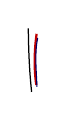
\begin{tikzpicture}[x=1em,y=1em,baseline=0pt]\draw[black,line width=.45pt] (.04,.2)..controls(.05,-.65)and(.08,-1.35)..(.16,-2.1);
\draw[red!75!black,line width=.8pt] (.34,0)..controls(.27,-.5)and(.23,-1.2)..(.33,-1.85);
\draw[blue!40!black,line width=.4pt] (.38,-.15)..controls(.25,-.7)and(.35,-1.55)..(.35,-1.92);\end{tikzpicture}}
\normalmarginpar
\[
\begingroup
\setbox0=\hbox{$\displaystyle\begin{array}{l}
\deleted{\unsure{\mathcal N_r(uv)|N_r(uv)}\leq\mathcal N_p(u)\mathcal N_q(v)}\\[.6ex]
\inserted{\|uv\|_r\leq\|u\|_p\|v\|_q}\quad\left(\frac1r=\frac1p+\frac1q\right)
\end{array}$}
\smash{\rlap{
\begin{tikzpicture}[x=\wd0,y=1ex,baseline=0pt]\draw[red!75!black,line width=1pt] (-.04,4.0)..controls(.18,3.8)and(.47,4.35)..(.72,4.3);
\draw[red!75!black,line width=1pt] (-.02,3.8)--(-.035,-3.2)..controls(.20,-3.4)and(.57,-2.9)..(1.05,-3.3);
\draw[red!75!black,line width=1.1pt] (1.02,2.5)..controls(1.05,1.4)and(1.02,-1.5)..(1.02,-3.2);
\draw[black,line width=.65pt] (.06,1.7)--(.045,.35)--(.20,3.25)--(.17,1.5)--(.30,3.8)--(.21,.1)--(.42,2.7)--(.36,.3)--(.50,2.35)--(.42,-.2)--(.58,1.25);
\draw[black,line width=.45pt] (-.04,-3.35)..controls(.27,-3.6)and(.66,-2.85)..(.96,-3.8);\end{tikzpicture}}}\box0
\endgroup
\]

\deleted{(\unsure{la somme} \illegible{3} \unsure{si tous les} \illegible{1})}

Le cas le plus important de l'inégalité (37) est celui où $s=1$, i.e. où $p$ et $q$ sont deux ``exposants conjugués''; \deleted{\unsure{Nous y reviendrons} \illegible{1}} \inserted{dans ce cas, (32) est d'ailleurs contenu dans} l'\deleted{\unsure{inégalité du|inégalités au} N\textsuperscript{o} suiv., en une formule plus frappante.}

\[
\begingroup
\setbox0=\hbox{$\displaystyle\|uv\|_1\leq\|u\|_p\|v\|_{p'}\quad\left(\frac1p+\frac1{p'}=1\right)$}
\begin{array}{ll}\textcircled{38}&\smash{\rlap{\begin{tikzpicture}[x=\wd0,y=1ex,baseline=0pt]\draw[red!75!black,line width=1pt] (.025,1.9)..controls(.27,2.3)and(.39,4.2)..(1.04,4.05);
\draw[red!75!black,line width=1pt] (-.025,1.75)--(-.05,-1.8)..controls(.25,-1.65)and(.58,.2)..(1.04,-.4);\end{tikzpicture}}}\box0\end{array}
\endgroup
\]

\deleted{(29) \unsure{qui est|si tous} : l'inégalité de Hölder \unsure{ordinaire}}. \inserted{(38) résulte d'ailleurs aussi de (32), grâce à l'inégalité de Hölder ordinaire}
\par\noindent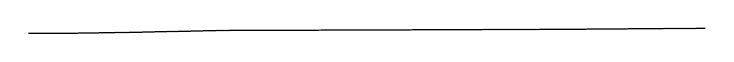
\begin{tikzpicture}[x=1cm,y=1ex,baseline=0pt]\draw[line width=.45pt] (0,0)..controls(.9,-.02)and(1.7,.15)..(2.6,.25)..controls(4.7,.28)and(6.6,.31)..(8.6,.42);\end{tikzpicture}

\reversemarginpar
\margin{\begin{tikzpicture}[x=1em,y=1em,baseline=0pt]\draw[line width=.5pt] (0,0)--(.5,.6);\end{tikzpicture}\par
Expliquer \unsure{l'itération|l'introduction} d'une \illegible{1}\par
\begin{tikzpicture}[x=1em,y=1em,baseline=0pt]\draw[line width=.55pt] (0,-.2)..controls(.65,.5)and(1.05,1.9)..(1.85,3.1);\end{tikzpicture}}
\normalmarginpar

\uline{Corollaire 4}. Soient $E,F,G$ trois espaces de Hilbert de $=$ dimension finie $n$, $u$ un op. cpt de $E$ dans $F$, $v$ un op. cpt de $F$ dans $G$, $f$ \inserted{$\unsure{(t_1,-t_n)|(s_1,-s_n)}$} une fonction \deleted{\unsure{sym.}} de $n$ arguments $t_i>0$ telle que $f(e^{t_{\unsure{i|1}}},-e^{t_n})$ soit fonction convexe de $(t_i)\in R^n$. Sous ces conditions, \inserted{si \deleted{\unsure{l'un de ces}} \inserted{$u$ et $v$} sont inversibles \unsure{ou|on a}} \deleted{la \unsure{formule}} \inserted{si $f$ est définie et continue pour $s_i\geq0$, on a}

\reversemarginpar
\margin{\textcolor{red!75!black}{\unsure{?}}\quad
\begin{tikzpicture}[x=1em,y=1em,baseline=0pt]\draw[red!75!black,line width=1.0pt] (0,.7)--(.12,-1.0);\end{tikzpicture}}
\normalmarginpar

\[
\begin{array}{ll}(39)&\displaystyle f(\rho_1(uv),-\rho_n(uv))\leq f(\rho_1(u)\rho_1(v),-\rho_{\unsure{n}}(u)
\end{array}
\]

En effet, \deleted{\unsure{on sait du}} \inserted{utilisant les conditions} du th. 1, 2\textsuperscript{o}, hyp. b),

\reversemarginpar
\margin{\uline{petits} \uline{caractères}}
\normalmarginpar

en vertu de

\[
\begin{array}{ll}(40)&\displaystyle\prod\rho_i(uv)=\deleted{f(uv)}\prod\rho_i(u)\rho_i(v)\end{array}
\]

\deleted{En effet,} \inserted{Pour vérifier (40),} on \deleted{\unsure{élève au carré}} \inserted{peut supposer} \deleted{est ramené} que $E=F=G$, alors les deux mb. de (35) sont resp\textsuperscript{t}. $|\det(uv)|$ et $|\det u|\,|\det v|$ (formule (\unsure{26|16})) d'où le résultat. Si $u$ et $v$ sont q.qcon\unsure{ques} mais $f$ définie et continue pour $t_i\geq0$, (39) sera encore valable par prolongement par continuité à partir du cas précédent.

Donner des liaisons sur la composition des opérateurs comme multiplication

\reversemarginpar\margin{93}\normalmarginpar
